
\chapter{Methodology and validation}

\section{Introduction}
 
An overview of the modeling and the computational methods used in this study are presented in this chapter. This study uses well established techniques to model and study fluid elastic galloping. Therefore, only a brief overview is provided together with relevant references where the development and vigorous validation has been presented.  

This chapter is presented as follows. The equations used to model the system are presented and discussed. Next, a brief discussion of the techniques used for direct numerical simulations are presented followed by the problem formulation and the discussion of the parameters used. Finally, validation data are presented and discussed to demonstrate the accuracy of the direct numerical simulations.


\subsection{Parameters used}

The findings in this study are presented in two categories i.e. high and low Reynolds numbers, so as to study the system at laminar and turbulent flow regimes. One of the main objectives in this study was to capture the flow physics accurately using direct numerical simulations. Hence, major portion of the study was carried out in the laminar range where the flow is laminar and two dimensional. Although a majority of the study is focused on low Reynolds number regime, some results were presented using inputs from published data at high Reynolds numbers to provide a comparison between high and low Reynolds number cases. $\reynoldsnumber=200$ was defined as the ``low" Reynolds number and $\reynoldsnumber=22300$ was defined as the high Reynolds number in this study. Studies by \citet{tong2008} and \citet{sheard2009} reveal that the approximate value of 3-dimensional transition of the wake for a square cross section is $\reynoldsnumber=160$ and therefore, $\reynoldsnumber=200$ was selected to represent the low Reynolds number regime, also considering the fact that other numerical studies in the laminar regime have used this value of Reynolds number \citep{Robertson2003,Joly2012}. All these published data have used a square cross section as the body of oscillation. Since the basic cross section used in this study is square, the same flow regimes of the these published data were used.

In the high Reynolds number case, the chosen Reynolds number matches the pioneering study of galloping \citet{Parkinson1964}, from which the stationary aerodynamic data was obtained as input to the QSS model. For the high \reynoldsnumber\ tests, predictions of power output at $\reynoldsnumber=22300$ were obtained using the coefficients of the $C_y$  vs. $\theta$ curve from \citet{Parkinson1964} as inputs to the QSS model. Aerodynamic data (i.e. \cy\ data) from direct numerical simulations at low Reynold number of stationary cases at different angles of attack are used as inputs to the QSS model at the low Reynolds number regime. 

Stationary $C_y$ data at different angles of attack is used as inputs to the QSS model, were obtained  for the low Reynolds number regime using direct numerical simulations. The average power was obtained by using equation \ref{eqn:power}, and the averaging was done over no less than 20 galloping periods. The mass ratio $m^*$ was kept at 1163 for $\reynoldsnumber=22300$ (Similar to \citet{Parkinson1964}). The parameters used at the low Reynolds number cases are $m^*=20$ for \reynoldsnumber=200 and $\ustar\geq 40$. These were similar to the parameters used in previous studies \citep{Robertson2003,Joly2012}. These parameters were used throughout this study unless specified otherwise.

\section{Quasi-steady model}
\label{sec:QSS_model_methodology}

The quasi-steady state model discussed in section \ref{sec:QSS theory} was used to obtain oscillator response data. The quasi-steady state model has proven its ability to obtain accurate galloping response data (as also discussed in section \ref{sec:QSS theory}). Therefore, a large number of cases can be modelled in small amount of computational time. The oscillator equation consists of spring, mass and damper oscillator expression with a $7^{th}$ order interpolation polynomial as the forcing function (equation \ref{final_equation_motion}), obtained from a curve fit of aerodynamic data (i.e. \cy\ as a function of the incidence angle).

\subsubsection{Solving the quasi-steady state equation}

The quasi-steady model being an ordinary differential equation can be solved using different solving methods. Some of the techniques include limit cycle oscillations, harmonic balance, cell mapping and numerical integration. \citet{Vio2007} showed that numerical integration provides accurate data. A fourth-order Runge-Kutta ODE solving scheme was used in solving the quasi-steady state oscillator equation. The built in `ode45' function in MATLAB was used primarily to solve the QSS equation while in some cases `ode15s' function was used when the equation became more stiff.


\section{Calculation of average power}
\label{subsec:ave_pow}
The ideal potential amount of harvested power output is represented as the dissipated power due to mechanical damping before losses in any power take-off system are included. Thus the mean power output can be expressed as 


\begin{equation}
\label{eqn:power}
P_{m}=\frac{1}{T}\int_{0}^{T}(c\dot{y})\dot{y} dt,
\end{equation}
where $T$ is the period of integration and $c$ is the mechanical damping constant. 

The work done on the body by the fluid is equal to this quantity, defined as
\begin{equation}
\label{eqn:power_alt}
P_{m}=\frac{1}{T}\int_{0}^{T}F_y\dot{y} dt,
\end{equation}
where $F_y$ is the transverse (lift) force.

The two definitions of the mean power provide two vital interpretations of power transfer. Equation \ref{eqn:power} shows that the power is proportional to the mechanical damping and the magnitude of the transverse velocity. At first glance one may assume that the power can be increased by increasing damping. In a practical power extraction device, the significant component of damping would be due to the electrical generator and therefore, an increase in damping would be due to the increase of the load or in other words the electrical resistance. Yet this perception of damping is not quite accurate as very high damping would result in reducing the velocity amplitude which then, would not result in a higher energy output according to equation \ref{eqn:power}. In consequence, a balance needs to be obtained where the damping is high, but not to the extent that it will adversely result by overly suppressing the motion of the body.  

On the other hand, equation \ref{eqn:power_alt} shows that a higher power is attained during situations where the transverse force $F_{y}$ and the transverse velocity are in phase. Hence, a simple increase in the magnitude of the force or the velocity is not satisfactory to attain a higher power transfer. A higher power output can be obtained when there is a smaller phase difference between the force and the velocity.   



\section{Direct numerical simulations (DNS)}

Direct numerical simulations were employed to obtain the stationary data to be used as inputs to the QSS model and to obtain  fluid-structure interaction (FSI) predictions to be compared with the QSS model at low Reynolds numbers. A high-order in-house build spectral element which simulates two-dimensional laminar flows was used to obtain the DNS data.


To obtain DNS results an in-house build code was used. This code essentially solves the Navier-Stokes equations in an accelerated reference frame. A three-step time-splitting scheme also known as a fractional step method was used for temporal discretisation. A predictor-corrector method was used for the FSI data where an elastically mounted body was involved. A description of the spectral element method in general can be found in \citet{karniadakis2005}. This code has been very well validated in a variety of fluid-structure interaction problems similar to that studied in the current study \citep{Leontini2007a,Griffith2011,Leontini2011,Leontini2013}. An overview of the algorithm is presented in the following subsections which is described in detail by \citet{Leontini:thesis}. 

\subsection{Governing equations}
 
  In this study, the following key assumptions were made to carry out the direct numerical simulations. 
 
 To formulate the differential equations to an infinitesimally small fluid section, the fluid was assumed to be a continuum. This assumption is valid for all macro flows as  is the case in this study. 
 
 
 Next, to avoid the modelling acoustic wave propagation, it was assumed that the density of the fluid is constant. The fluid is incompressible. This particular assumption is usually valid for Mach numbers (ratio of the speed of sound to the speed of fluid flow ) less than 0.3.
 
 Finally, the fluid was assumed to be an Newtonian fluid, which means that the shear stress is directly proportional to the strain rate.The assumptions used are quite standard and further information can be found in \citet{White99}.        

The Navier-Stokes equations are the equations which governs a Newtonian, incompressible fluid.
  \begin{equation} \centering
  \label{eq:nsdim}
  \pderiv{\vecu}{t} + (\vecu\cdot\nabla)\vecu\ = -\frac{\grad{\pres}}{\density} + \frac{\dynvis}{\density}(\gradsq{\vecu})~,
  \end{equation}
  and continuity,
  \begin{equation} \centering
  \divergence{\vecu} = 0~.
  \end{equation}
  
  The velocity vector field is represented by \vecu, time by $t$, the pressure field by \pres \ fluid density by \density \ and the dynamic viscosity by \dynvis. In the Navier-Stokes equation (\ref{eq:nsdim}) the left hand side represents the inertial forces and the right hand side represents the pressure forces. The net mass flux into the fluid element is specified to be zero by the continuity equation. 
  
  These equations are generalised by non-dimensionalisation. In the case of bluff body wake flows, the equations are non-dimensionalised by using the characteristic length of the body i.e the frontal projected hight \diam, and the free-stream velocity \Ufree. 
  
  For cases investigating fluid structure interactions the equations are modified  to  be solved in an accelerated reference frame. The frame of reference is attached to the cylinder. Therefore, an extra term is added to the Navier-stokes equations which represents the acceleration of the cylinder. Thus, the equations can be written as, 
  
  \begin{equation} \centering
  \label{eq:nsfinal}
  \pderiv{\vecV}{\tau} = -\grad{\Pres} + \frac{1}{\Rey}(\gradsq{\vecV}) - (\vecV\cdot\nabla)\vecV + \accframe ~,
  \end{equation}
  \begin{equation}
  \label{eq:continuity}
  \divergence{\vecV} = 0~.
  \end{equation}
  
   The non dimensional terms are defined s follows: $\vecV = \vecu/U$, $\tau = tU/D$, $\Pres = \pres/(\density
  U^{2})$, $\Rey = \density UD/(\dynvis)$, $\Vcyl = \vcyl/U$, and 
  $\vcyl$ being the velocity of the cylinder. \accframe, represents acceleration of the cylinder.  
  
  The Navier-Stokes equations are coupled with the oscillator differential equation 
  
  \begin{equation} \centering
  \label{eq:cyl_eom}
  \frac{\ddot{y}_{cyl}}{D} + 2\damping\sqrt{\kstar}\frac{\dot{y}_{cyl}}{D} + \kstar\frac{\ycyl}{D} = \frac{\pi}{2}\frac{\clift}{\mstar} ~,
  \end{equation}

  
    Where \damping \ is the damping ratio,  $\kstar=kD^{2}/m\Ufree^{2}$ and
    $\clift = \liftf/(0.5\density U^{2}D)$. The lift
    coefficient per unit length of the body is \clift, the transverse displacement of the cylinder is given by \ycyl,  the characteristic length scale of the body is $D$, $k$ is the spring constant and the mass per unit length of the body is represented by $m$. The general form of this linear oscillator equation can be found in books such as  \citet{Naudasher94}. The final form of the coefficients were constructed by non-dimensionalising the general linear oscillator equation. 
    
    
 
 \subsection{Temporal discretisation: Time-splitting}
 
 The problem was discretised in order to solve equations \ref{eq:nsfinal}, \ref{eq:continuity} and \ref{eq:cyl_eom} in both space and time. A three-step time splitting method was used for the temporal discretisation. This scheme also known as the fractional step method, was used to separately integrate the terms in the right hand side of the Navier-Stokes equation \citep{karniadakis2005}. The overall integration of one time-step is split into three substeps. An approximate solution of the Navier-Stokes equation is gained by this scheme. 
 
 The cylinder acceleration is integrated through the whole time step in order to obtain an initial approximation of the intermediate velocity filed. This velocity filed is used as the starting condition. The pressure is integrated using this starting condition.  A secondary intermediate velocity filed is obtained as a result of the pressure integration substep. This secondary velocity filed is then used as the starting condition for the integration of the diffusion term which results in the final velocity filed. 
 
 The three semi-discretised substep equations are as follows:
 
\begin{equation} \centering
\label{eq:substep1}
\Vint - \Vn - \Delta\Vcyl = -\int_{\tau}^{\tau+\Delta\tau}(\vecV\cdot\nabla)\vecV \mathrm{d}\tau
\end{equation}
\begin{equation} \centering
\label{eq:substep2}
\Vintint - \Vint = -\int_{\tau}^{\tau+\Delta\tau}\nabla\Pres \mathrm{d}\tau
\end{equation}
\begin{equation} \centering
\label{eq:substep3}
\Vnext-\Vintint = \frac{1}{\Rey}\int_{\tau}^{\tau+\Delta\tau}\gradsq{\vecV} \mathrm{d}\tau,
\end{equation} 
 
The current time step is represented by $n$ and the intermediate velocity fields at the end of the convection and pressure substeps are $\Vint$ and $\Vintint$ respectively. The change in the body over a time step is given by $\Delta\Vcyl =
\int_{\tau}^{\tau+\Delta\tau}\accframe \mathrm{d}\tau$. 

The addition of these three substep equations reduces to the integrated form of the Navier-Stokes equation in equation \ref{eq:nsfinal}. 

\subsubsection{Integration of the substep equations}
\label{subsec:sol}
 
 The integration methods of the pressure, convection and diffusion substeps are presented in this subsection. 
 
 \subsubsection{The convection substep}
 \label{subsub:convec}
 
As the system involves free oscillation, a coupling between the oscillation equation (equation \ref{eq:cyl_eom}) and the Navier-Stokes equations had to be employed. As a result, the cylinder dynamics had to be solved at each time-step.

An iterative predictor-corrector scheme was employed to obtain the solution of the coupled equations. The initial step being the ``predictor" step was obtaining approximations for all the quantities involved in  the integration. A quadratic extrapolation was used to obtain an initial estimate of $\Delta\Vcyl$ from  three previous time step values of $\Vcyl$. Therefore, a non-dynamical approximation can be obtained.  
 
 
\begin{equation} \centering
\label{eq:vcyl_start}
\Vcyl^{(n+1)\dag} = 3\Vcyl^{(n)} - 3\Vcyl^{(n-1)} + \Vcyl^{(n-2)} ~,
\end{equation}


The dagger ($\dag$) indicates that the value is an initial approximation eg. $\Vcyl^{(n+1)\dag}$. Thus, $\Delta\Vcyl^{\dag}$ was obtained by a simple subtraction of the value at the current time step. 

The approximated position of the cylinder at the next time step can be obtained by carrying out an integration of the cylinder velocity over the time step. A third-order Adams-Moulton method was used to perform the integration. Therefore, the final equation describing the position of the body is given by, 

\begin{equation} \centering
	\label{eq:ycyl_start}
	\frac{\ycyl^{(n+1)\dag} - \ycyl^{(n)}}{\Delta\tau} = \frac{1}{12}(5\Vcyl^{(n+1)\dag} + 8\Vcyl^{(n)} -  
\end{equation}

The transverse displacement of the cylinder is denoted by \ycyl.

An offset is present between the cylinder velocity and cylinder position. The velocity of the cylinder is in advance by half a time-step of the position of the cylinder, i.e. $\Vcyl^{(n+1)}$ is half a time step is in advance of $\ycyl^{(n+1)}$. However, both the cylinder positions and the velocities are located at the same discrete times.

In order to obtain an approximation for \Vint, a solution was obtained for equation \ref{eq:substep1} using the previous approximated quantities.

By using a third-order Adams-Bashforth scheme and incorporating the approximation of equation \ref{eq:vcyl_start} for  $\Delta\Vcyl^{\dag}$ the first approximation for $\Vint$ was obtained using the equation,
 
\begin{equation} \centering
\label{eq:vint_first}
\frac{\Vint - \Vn - \Delta\Vcyl^{\dag}}{\Delta\tau} = \frac{1}{12}(23\mathbf{N}(\vecV)^{(n)} - 16\mathbf{N}(\vecV)^{(n-1)} + 5\mathbf{N}(\vecV)^{(n-2)}) ~.
\end{equation}

The explicit integration method was only used for the first approximation and for the subsequent iterations semi-implicit method was used for $\Vint$.

This step was followed by solving the remaining substep equations in order to obtain an approximation for  $\vecV^{(n+1)\dag}$, and then the ``predictor'' portion of the predictor-corrector method was completed.

The cylinder velocity approximation $\Vcyl^{\dag}$, was updated commencing the ``corrector'' cycle of the predictor-corrector method. This was carried out using a third-order integration scheme. 

 \begin{equation} \centering
 \label{eq:vcyl_correct}
 \frac{\Vcyl^{(n+1)\dag} - \Vcyl^{(n)}}{\Delta\tau} = \frac{1}{24}(25\ddot{y}_{cyl}^{(n+1)} - 2\ddot{y}_{cyl}^{(n)} + \ddot{y}_{cyl}^{(n-1)}) ~.
 \end{equation}
 
 $\Delta\Vcyl^{\dag}$ was updated using the recalculated value of $\Vcyl^{(n+1)\dag}$. The velocity was integrated over a time step in order to obtain the position of the cylinder. For the first correction cycle a third order Adams-Moulton method was used which completed the first iteration of the predictor-corrector method. 
 
 \begin{equation} \centering
 \label{eq:ycyl_correct}
 \frac{y^{(n+1)\dag} - y^{(n)}}{\Delta\tau} = \frac{1}{12}(5\Vcyl^{(n+1)\dag} + 8\Vcyl^{(n)} - \Vcyl^{(n-1)}) ~,
 \end{equation}
 
 Slight modifications were employed to the subsequent iterations in order to improve numerical stability. However, the iterations proceeded in a similar manner. As the approximations for  $\Delta\Vcyl^{\dag}$ and $\vecV^{(n+1)\dag}$  were available, further correction steps were carried out using third-order Adams-Moulton scheme . 
 
 \begin{equation} \centering
 \label{eq:predict_general}
 \frac{\Vint - \Vn - \Delta\Vcyl^{\dag}}{\Delta\tau} = \frac{1}{12}(5\mathbf{N}(\vecV)^{(n+1)\dag} + 8\mathbf{N}(\vecV)^{(n)} - \mathbf{N}(\vecV)^{(n-1)}) ~.
 \end{equation}
 
 The two remaining substeps were then solved to obtain a new approximation of $\vecV^{(n+1)\dag}$. 
 
 The first correction step was carried out by employing \ref{eq:vcyl_correct} to obtain a second estimate for the velocity of the cylinder $\Vcyl^{(n+1)\ddag}$. A relaxation equation (equation \ref{eq:relax}) was used for the velocity of the cylinder prior to using equation \ref{eq:ycyl_correct} since the equations were quite stiff.
 
 \begin{equation} \centering
 \label{eq:relax}
 \Vcyl^{(n+1)\prime} = \Vcyl^{(n+1)\dag} + \epsilon(\Vcyl^{(n+1)\ddag} - \Vcyl^{(n+1)\dag}) ~,
 \end{equation}
 
 $\Vcyl^{(n+1)\ddag}$ and $\Vcyl^{(n+1)\dag}$ represent the most current and previous approximations respectively. The under relaxation parameter is represented by $\epsilon$ which controls the proportion of the correction which is considered in each iteration. The final approximation at the end of the relaxation process is represented by $\Vcyl^{(n+1)\prime}$ and was used in equation \ref{eq:ycyl_correct} for completing the correction cycle and hence, the iteration.
 
  A convergence error criteria was specified until which the iteration was continued. The lift force of the cylinder, the velocity of the cylinder and the fluid velocity should all converge to the required convergence criteria. A series of convergence studies were carried out in order to obtain the convergence criteria \citep{Pregnalato:thesis}. The solution converged typically within $3-4$ iterations and the iteration count exceeded $10$ in very rare cases.  
  
  The procedure to obtain the solution for $\Vint$ (velocity filed at the end of the convection subsetep) in a nutshell is as follows. A predictor-corrector method was employed, where the primary predictor cycle was first employed. This was followed by obtaining an approximation for $\Delta\Vcyl$ which was calculated using equation \ref{eq:vcyl_start}. From this approximation ($\Delta\Vcyl$)  the position of the cylinder was approximated using equation \ref{eq:ycyl_start}.
 
 Next, using an explicit Adams-Bashforth scheme, an approximation was obtained for $\Vint$ by solving the substep equation (equation \ref{eq:vint_first}). The predictor cycle was completed by solving the remaining substep equations to arrive at the first approximation of \Vnext.   
 
 Then, the primary corrector step was initiated by calculating the forces of the body from the current approximation of \Vnext. Using these forces together with the current approximations of the velocity and the displacement of the body and the equation of motion of the body (eq:\ref{eq:cyl_eom}) an approximation for the acceleration of the cylinder at the end of the timestep was obtained. By integrating this acceleration over the timestep using equation \ref{eq:vcyl_correct} the corrected approximation of $\Delta\Vcyl$ was obtained. Using equation \ref{eq:ycyl_correct} the corrected approximation for $\ycyl^{(n+1)}$  was obtained by integrating the velocity over a timestep and using the recent value of $\Delta\Vcyl$. The primary corrector step and the primary iteration was completed once this step was completed. All the remaining iterations were carried out in a similar manner with an under relaxation presented in equation \ref{eq:relax}. 
 
 
\subsubsection{The pressure substep}

The pressure equation was solved in two parts in order to find solutions to the two unknowns i.e. the pressure filed and the velocity filed at the end of the timestep. 
 
The integration of the pressure substep was initiated by formulating equation \ref{eq:substep2} in terms of a second-order Adams-Moulton scheme which gives,
 
\begin{equation} \centering
\label{eq:pres_num}
\frac{\Vintint - \Vint}{\Delta\tau} = -\frac{1}{2}(\grad\Pres^{(n+1)} + \grad\Pres^{(n)}) ~.
\end{equation}

The equation was further reduced by considering that the $RHS$ is equal to $\grad\Pres^{(n+1/2)}$. The divergence portion of equation \ref{eq:pres_num} was taken. Using equation \ref{eq:continuity}, continuity was applied to the velocity filed which resulted the pressure filed having a Poisson equation of the form of 

\begin{equation} \centering
\label{eq:poisson}
\gradsq\Pres^{(n+\frac{1}{2})} = \frac{1}{\Delta\tau}\divergence{\Vint} ~.
\end{equation} 

This equation can be solved at the middle of the timestep for the pressure filed. Therefore, this pressure filed can then be back-substituted to equation \ref{eq:pres_num}, together with the simplified $RHS$, to solve for the velocity filed \Vintint, at the end of the substep. 

\subsubsection{The diffusion substep}

A numerical stability of the solution scheme has to be considered for the diffusion substep although the equation for diffusion is linear. Therefore, the Crank-Nicholson scheme or the second order Adams-Moulton scheme which is a semi-implicit scheme and unconditionally numerically stable is employed. Thus this formulates the final equation (eq \ref{eq:substep3}) of the time splitting scheme as,

\begin{equation} \centering
\label{eq:diff_num}
\frac{\Vnext - \Vintint}{\Delta\tau} = \frac{1}{2\Rey}(\gradsq{\Vnext} + \gradsq{\vecV^{(n)}}) ~.
\end{equation}

The integration over the timestep is obtained from the solution of this equation  for \Vnext, thus completing the time splitting scheme. 


\subsubsection{Spatial discretisation:Spectral element method}
 
 The spatial discretisation was done using a nodal based spectral-element method. This method is a member of the finite-element class. The computational domain is separated into a series of macro elements and then a continuous solution is obtained over each element. Mesh refinement can be done in the areas where high gradients are experienced, which is also known as $h$-refinement. It was necessary that all elements to be quadrilateral. Yet, the elements were not restricted from having curved sides.
 
 The calculation of the residual \residual\ initiates the solution process. All the terms of the governing equations (the Navier-Stokes equation eq \ref{eq:nsfinal}) were moved to the $LHS$. Thus, the resulting expression is, 
 
 \begin{equation} \centering
 \label{eq:ns-oneside}
 \pderiv{\vecV}{\tau} + \grad{\Pres} - \frac{1}{\Rey}(\gradsq{\vecV}) + (\vecV.\nabla)\vecV - \accframe = 0 ~.
 \end{equation}
 
 A trial solution is substituted into equation \ref{eq:ns-oneside}. The $RHS$ of the equation would be zero if the trial solution is the exact solution of the equation. If the trial solution is not the exact solution but an approximation to the exact solution which is the case in general, then the $RHS$ will be non-zero and a residual will be formed. This residual can be defined by, 
 
 \begin{equation} \centering
 \label{eq:residual}
 \pderiv{\Vtrial}{\tau} +\grad{\Ptrial} - \frac{1}{\Rey}(\gradsq{\Vtrial}) + (\Vtrial.\nabla)\Vtrial - \accframe = \residual ~,
 \end{equation}
 
 The trial solutions for velocity and pressure fields are \Vtrial\ and \Ptrial\ respectively. The error term which is introduced through the trial function is the residual \residual. It is clear from equation \ref{eq:residual} that the definition of the residual is the governing equation substituted by the trial solution substituted to the true solution.
 
In order to effectively distribute the error over the domain, the residual has to be weighted in order to minimise the maximum local error. To perform this task the inner product of the residual with a series of weighing functions were taken. The integral of the product of the weighting  function and the residual is the inner product of the residual which is set to zero. The method employed here is also commonly known as weighted residual method. 

Tensor-product Lagrange polynomials were used for both interpolating trial functions and weighting functions in the DNS carried out in this study. The order of the polynomials $p$ can be varied from $2$ to $14$ in order to further improve grid resolution which is also known as $p$ refinement. This $p$ refinement coupled with $h$ refinement leads to a method called $h-p$ method which is used to improve accuracy \citep{karniadakis2005}. The method also can be referred as a Galerkin method as both trial and weighting functions used were from the same family of functions. \citet{Fletcher84,Fletcher91} provides further details on weighted-residual methods and Galerkin method. 

Lagrange polynomials can be defined as, 

\begin{equation} \centering
\label{eq:lagrange}
L_{i}(\compone) = \underset{g\neq i}{\prod_{g=1}^{p+1}}\frac{(\compone-\compone_{g})}{(\compone_{i}-\compone_{g})}
\end{equation}

The spatial coordinate is $\compone$ and the indices of the data points are represented by $i$ and $g$ and the number of data points are represented by $p+1$. One of the properties of Lagrange polynomials is that being equal to unity at the point $i$ and being zero at all the other points other than in places in between points. Thus a continuous polynomial which matches the exact values of the velocity at the node point  can be obtained when  $L_{i}$ is multiplied by the velocity at point $i$ and then summing over all points. The tensor-product polynomials in two dimensions $N_{q,s}(\compone, \comptwo)$ can be defined as the product of the Lagrange polynomial in one direction $L_{q}(\compone)$, with that in the other direction .$L_{q}(\comptwo)$ 

The outline of the procedure to find the solution is as follows. The process is initiated by forming inner product of the residual and the tensor-product Lagrange polynomial weighting function.

This gives the integral 

 \begin{equation} \centering
 \label{eq:inner-prod}
 \int\int_{\Omega}N_{k,m}(\compone,\comptwo)\cdot[\pderiv{\Vtrial}{\tau} +\grad{\Ptrial} - \frac{1}{\Rey}(\gradsq{\Vtrial}) + (\Vtrial\cdot\nabla)\Vtrial - \accframe]\mathrm{d}x\mathrm{d}y = 0 ~,
 \end{equation}
 
The computational domain is represented by $\Omega$. $N_{q,s}(\compone,\comptwo)$ are the weighting function as defined in the computational space.

From equation \ref{eq:inner-prod} it is shown that each term in the equation is multiplied by the weighting function. Thus, the integral is split into components and the process can be carried out in the each of the substep equations \ref{eq:substep1}, \ref{eq:substep2} and \ref{eq:substep3}. For example the discretised equation for \ref{eq:vint_first} can be expressed as

\setlength{\multlinegap}{0.2\textwidth}
\begin{multline} 
\label{eq:inner_conv_osci}
\frac{1}{\Delta\tau}\int\int_{\Omega}N_{q,s}(\compone,\comptwo)\cdot(\Vtrial^{*} - \Vtrial^{(n)} - \Delta\Vcyl)\mathrm{d}x\mathrm{d}y = \\
\int\int_{\Omega}N_{q,s}(\compone,\comptwo)\cdot(\frac{1}{12}(23\mathbf{N}(\Vtrial)^{(n)} - 16\mathbf{N}(\Vtrial)^{(n-1)} + 5\mathbf{N}(\Vtrial)^{(n-2)}))\mathrm{d}x\mathrm{d}y ~.
\end{multline}

 This integral can be broken into components. Hence, the first term of the of the LHS of equation \ref{eq:inner_conv_osci} can be defined as,  
\begin{equation} \centering
\label{eq:inner_real}
\int\int_{\Omega}\Vtrial^{*} N_{q,s}(\compone,\comptwo)\mathrm{d}x\mathrm{d}y ~.
\end{equation}

% % % % % % % % % %

The first term in equation \ref{eq:vint_first} can be used as an example to illustrate the process of obtaining the solution using the spectral element method. In order to calculate the integral of equation \ref{eq:inner_real}  over the entire computational domain, the integral is evaluated over each element separately. After that, the contributions of each element are summed together. 

All the quadrilateral elements are mapped to a square ranging between $-1,1$ in both directions where \compone\ and \comptwo\ are the orthogonal coordinates of this square. The approximation of the integral is simplified by defining the internal node points with the Gauss-Lobatto-Legendre (GLL) quadrature.

A Jacobian is introduced to perform this coordinate transformation and hence, the integral over each element becomes,
\begin{equation} \centering
\label{eq:inner_comp}
\int\int_{El}\Vint N_{q,s}(\compone,\comptwo)\jacobian(\compone, \comptwo)\mathrm{d}\compone \mathrm{d}\comptwo ~,
\end{equation}

The Jacobian represented by \jacobian and ``$El$" denotes that the integration is performed over a single element. The solution of equation \ref{eq:inner_comp} $\Vtrial^{*}$, can be re-written as a summation of Lagrange polynomial components. This equation also expresses the tensor-product Lagrange polynomials representing the weighting functions in directions of \compone\ and \comptwo. Therefore, the equation can be expressed as,    

 \begin{equation} \centering
 \label{eq:inner_expand}
 \int\int_{El}\sum_{i,j}\widehat{\Vint}L_{i}(\compone)L_{j}(\comptwo)L_{q}(\compone)L_{s}(\comptwo)\jacobian(\compone, \comptwo)\mathrm{d}\compone \mathrm{d}\comptwo ~.
 \end{equation}
 
 The velocity in the nodal points are represented by $\widehat{\Vint}$, $L$ is the one-dimensional Lagrange polynomial and $i$ and $j$ represents the node index in directions \compone\ and \comptwo. 

The Gauss-Lobatto Legendre (GLL) quadrature can be used to obtain an approximation to the integral in equation \ref{eq:inner_expand}, taking the definition of the location of the internal points in the computational domain. Thus approximation of \ref{eq:inner_expand} can be expressed as,

\begin{equation} \centering
\label{eq:inner_GLL}
\sum_{a,b}W_{a,b}\sum_{i,j}\widehat{\Vint}_{i,j}L_{i}(\compone_{a})L_{j}(\comptwo_{b})L_{q}(\compone_{a})L_{s}(\comptwo_{b})\jacobian(\compone_{a}, \comptwo_{b}) ~.
\end{equation}

$W_{a,b}$ represents the weighting coefficient for GLL quadrature, $a$ and $b$ represents the position of the node in the directions \compone\ and \comptwo\ respectively. 


Even though equation \ref{eq:inner_GLL} appears to be quite intimidating to deal with, the expression can be considerably simplified because of the fact that the system is discrete and the only values at the nodal points are considered. Incorporating Lagrange polynomials allows the substitution 

 \begin{gather}
 \label{eq:kronecker}
 \L_{i}(\compone_{a}) = \delta_{ia} = \begin{cases}
 1 & i = a    \\
 0 & i \neq a \\
 \end{cases} ~.
 \end{gather}
 
 The Kronecker delta is expressed by $\delta_{ia}$. This substitution leads to a significant reduction of the non-zero elements in the simulation and leads to a much simpler expression. If the convection substep (example considered here) is considered, only a single term remains based on the \Vint\ term in the convection substep equation which is,


 \begin{equation} \centering
 W_{q,s}\jacobian(\compone_{q},\comptwo_{s})\widehat{\Vint}_{q,s} ~.
 \end{equation}
 
 
 All the governing terms can be simplified similarly and this process is repeated over all elements. A global matrix is assembled by collecting the contribution of each element and then this matrix system is solved to obtain solution for the unknown velocity and pressure fields at the nodal points. 
 
 Only the continuity of each function is required across the boundaries, with no condition imposed on the gradient (this condition
 is known as $C_{0}$ continuity), even though the shape functions are higher-order polynomials within each element. It can be shown that the method achieves global exponential convergence \citep{karniadakis2005}.  
 
 The numerical process used for this study has been demonstrated to give
 exponential spatial convergence as the number of internal nodes per
 element is increased \citep{Thompson1996a}.
 


\subsubsection{Boundary conditions}

The boundary conditions, regardless of the mesh  were common for all the simulations performed. A no-slip condition was applied to the cross section wall. This condition ensures that the velocity is zero at the surface of the cross section. For stationary simulations a Dirichlet boundary condition is applied. For FSI cases a time-dependent Dirichlet boundary condition was employed for the velocity on the inlet and lateral boundaries. A Dirichlet boundary condition should have a specified value for the variables \citep{kreyszig2010} in this case velocity. The time-dependent Dirichlet condition has to be implemented for the FSI cases to account for the accelerated reference frame attached to the cross section. Thus, the inlet boundary was set to $u=U$ and $v=-\dot{y}$ for FSI cases and $v=0$ for stationary cases, where $u,v$ are the velocities in the $x$ and $y$ directions, respectively.


The outlet which is at the boundary downstream of the body was assigned the Neumann boundary condition (where the gradient of a property is specified \citet{tu2007}), $\pderiv{\vecV}{\normal}=0$ where \normal\ denotes the unit normal vector. This assumes that the flow does not spatially evolve while exiting the domain.



% % % % % % % % % % % % %

A Neumann condition for the pressure was applied at all the boundaries except the outlet. The normal gradient was calculated from the Navier--Stokes equations. A Dirichlet condition for the pressure ($p=0$ was enforced at the outlet. The details of the method can be found in \citet{Thompson2006,Thompson1996a}

 Although the physical validity of the outlet boundary condition is not quite true, this does not turn out to be a significant problem provided that the Reynolds numbers are low and the domain is sufficiently far away from the body.


 % % % %what exacly was used ?????????

% % % % % % % % % % % % % % % %
 
 
 
 
 
 
\subsection{Convergence and validation studies}

\subsubsection{Domain size}

A numerical domain similar to \citet{Leontini2013} was used  as the numerical domain in the present study where the trailing part of the domain was increased to capture the long wave lengths of flow frequencies. This selection was done for two reasons, one being both studies \citet{Leontini2013} and the present study interoperates the same numerical solving code and the other being the cross sections carried out in both studies are similar. Thus, further optimisation of the domain need not be carried out as \citet{Leontini2013} has already been optimized for the accuracy. \KJ{justin: I think I have to re-word this let me know whether you get the idea of what I am trying to say here and provide me some points to improve this paragraph}

For all cases, a rectangular domain was employed where the inlet was placed $20D$ from the centre of the body, while the outlet was situated $60D$ away from the centre of the body. The lateral boundaries were placed $20D$ away from the centre of the body. The macro element arrangement of the general domain is shown figure \ref{fig:square-mesh}. The macro element arrangement near the cross section was altered to cater for different cross sections. The near wall macro element configuration for the different cross sections are presented in figure \ref{fig:zoom-mesh}.The domain incorporated was essentially similar to the domain used in \citet{Leontini2013} apart for the long trailing section to capture the long wavelengths of galloping frequencies. 
 
 \begin{figure}[h!]
\setlength{\unitlength}{\textwidth}

  \begin{picture}(0.95,0.5)(0,0.8)
   
  \put(0.2,0.76){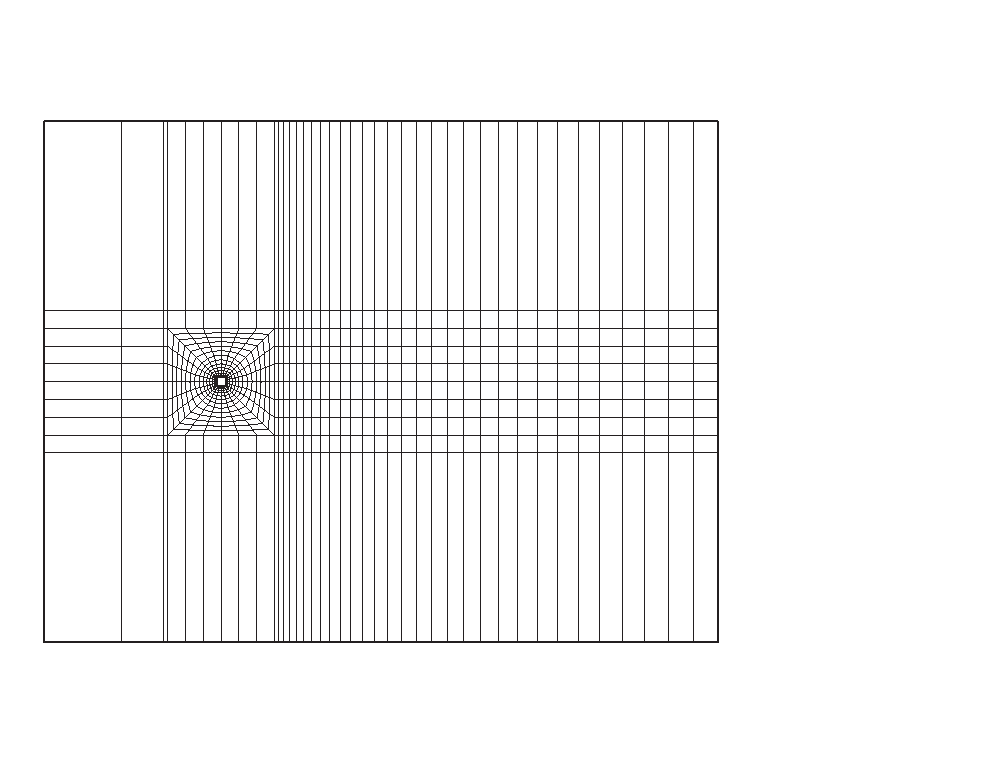
\includegraphics[width=0.8\unitlength]{./chapter-methodology/fnp/square-mesh.eps}}         
      
      
   

      	

  \end{picture}

 \caption{Macro element arrangement in the domain for the square cross section geometry. The inlet extending  $20D$ upstream from the centre of the body, while the outlet extends $60D$ downstream from the centre of the body. The lateral boundaries were placed $20D$ away from the centre of the body.}
    \label{fig:square-mesh}
\end{figure}
 
 
 \begin{figure}
  \setlength{\unitlength}{\textwidth}
\fbox{
  \begin{picture}(0.95,1.3)(0,0.7)
    % % %90
      % % % Parkinson Data 
      \put(0.035,1.65){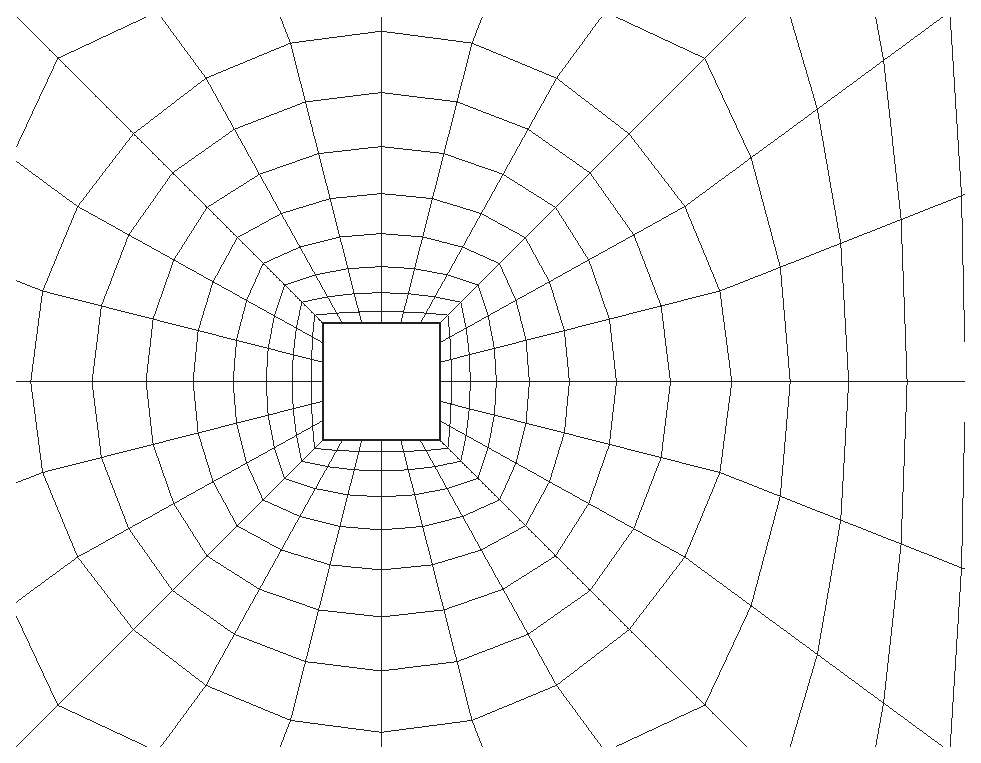
\includegraphics[width=0.4\unitlength]{./chapter-methodology/fnp/mesh.eps}}
      \put(0.495,1.65){\includegraphics[width=0.4\unitlength]{./chapter-methodology/fnp/{hyb0.75-mesh}.eps}}
      \put(0.035,1.25){\includegraphics[width=0.4\unitlength]{./chapter-methodology/fnp/{hyb0.5-mesh}.eps}}
      \put(0.495,1.25){\includegraphics[width=0.4\unitlength]{./chapter-methodology/fnp/{hyb0.25-mesh}.eps}}
      \put(0.3,0.85){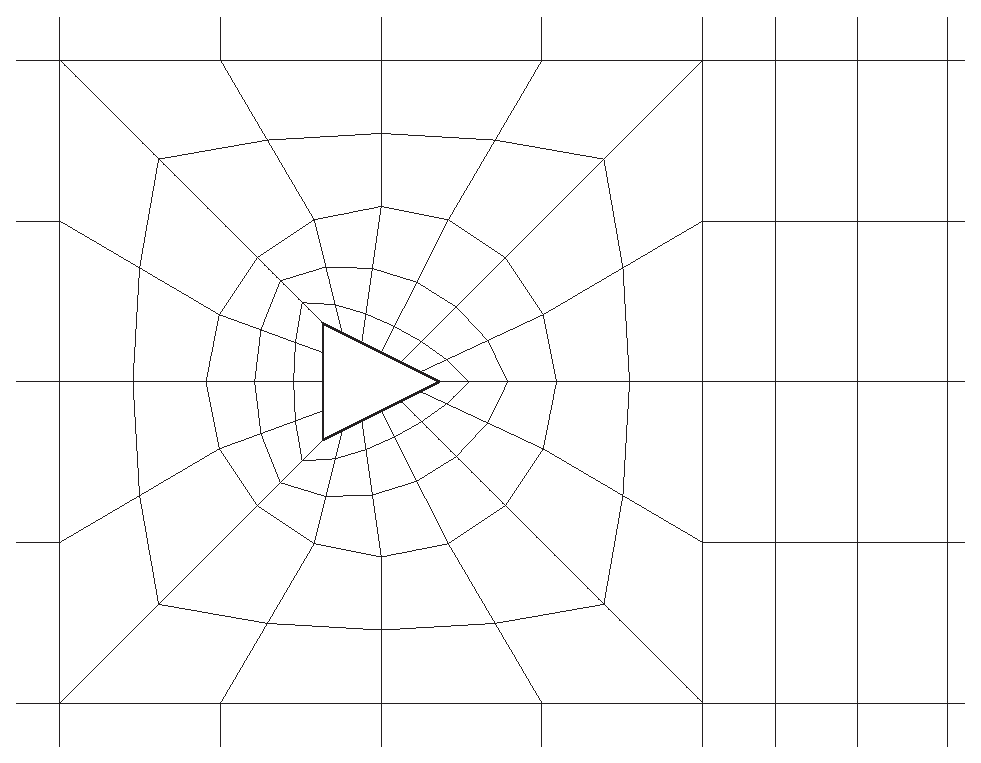
\includegraphics[width=0.4\unitlength]{./chapter-methodology/fnp/triangle-mesh.eps}}
      
      
   
      
      
%      \put(0.23,0.00){ $\displaystyle\frac{c}{\rho\mathcal{A}U}$}
%      \put(0.73,0.00){ $\displaystyle\frac{c}{\rho\mathcal{A}U}$}

     
      \put(0.206,1.605){\small(a)}
      \put(0.665,1.605){\small(b)}
      \put(0.206,1.2){\small(c)}
      \put(0.665,1.2){\small(d)}
      \put(0.45,0.8){\small(e)}
      

  \end{picture}
}
\caption{Configuration of the macro elements near the cross section. (a) square, (b) $\ratio=0.75$, (c) $\ratio=0.5$, (d) $\ratio=0.25$ and (e) triangle.}
  
  \label{fig:zoom-mesh}
\end{figure}

\subsubsection{Convergence}

A series of simulations for the oscillatory cases were carried out in order to ensure the results were grid independent. This was done by by keeping the layout of the macro element the same and varying the order of the interpolation polynomial (\emph{p-refinement}). The displacement amplitudes were compared against various polynomial orders. The time step is also reduced as the spectral resolution increases to satisfy the Courant condition. The summary of the results are presented in figure \ref{fig:FSI_convergence} .

% !TeX spellcheck = en_GB
\begin{figure}
  \setlength{\unitlength}{\textwidth}

  \begin{picture}(1,0.3)(-0.02,0)
          
    \put(-0.02,0.04){\includegraphics[width=0.5\unitlength]{./chapter-methodology/fnp/vel-amp-convergencexs.eps}}
    \put(0.5,0.04){\includegraphics[width=0.5\unitlength]{./chapter-methodology/fnp/freq-response-convergencexs.eps}}
        
    \put(0.48,0.166){ $ f_{DNS}$ }
    \put(-0.03,0.166){$\displaystyle\dot{y}_{m}$}
    % \put(0.73,0.00){ $\displaystyle\frac{c}{\rho\mathcal{A}U}$}

    \put(0.23,0.03){\emph{p-order}}
    \put(0.75,0.03){\emph{p-order}}
   
    \put(0.071,0.24){\small(a)}
    \put(0.605,0.24){\small(b)}
      
    \end{picture}

    % \caption{Comparison of DNS data. (a) Maximum power obtained using
    %   a 3 point localised quadratic fitting as a function of
    %   \massstiff. (b) \massdamp as a function of \massstiff at maximum
    %   power}

    \caption{Mean velocity amplitude ($\dot{y}_{m}$) (a) and the galloping frequency ($f_{DNs}$) (b) as a function of the interpolation polynomial. Data present $\frac{tU}{D}=0.001$ (\ding{83}) and $\frac{tU}{D}=0.0005$ ($\bullet$). Data acquired  $\reynoldsnumber=200$ $\massdamp=0$ using FSI direct numerical simulations.}

    \label{fig:FSI_convergence}
\end{figure}

 %vspace{10cm}


Figure \ref{fig:FSI_convergence} shows the mean velocity amplitude (sub-figure (a)) and the galloping frequency (sub-figure (b)) at different polynomial orders. Two factors namely, the quantitative accuracy of the data and the computational time had to be considered during the decision making process to obtain the optimum spacial and temporal resolution. Even though higher order polynomials gave very accurate data, the time step has to be reduced accordingly to meet the Courant condition. As galloping is a low frequency phenomenon, a longer time is taken to achieve the steady oscillating state. Furthermore, as galloping is dependent on the initial excitation of the flow, the initial development of galloping takes a significant amount of time. Both of these factors result in long computation times raging from 1 to 2 weeks or more. Thus a $9^{th}$ order polynomial was incorporated with $\frac{tU}{D}=0.001$ time-step. which produced an acceptable computation time with an acceptable accuracy. A difference of less than $1\%$ was achieved for both mean velocity amplitude  of the body and galloping frequency using this spatial and temporal parameters.

For the static cases a $11^{th}$ order polynomial was incorporated with $\frac{tU}{D}=0.00025$ time-step to ensure high accuracy as these parameters were beyond the parameters used in \citet{Leontini2013} (\KJ{time-step and polynomial}).


The FSI simulations for other cross sections presented in this thesis were also carried out using these special and temporal parameters.     















